


% Chapter Template

\chapter{State of the Art} % Main chapter title

\label{Chapter2} % Change X to a consecutive number; for referencing this chapter elsewhere, use \ref{ChapterX}

%----------------------------------------------------------------------------------------
%	SECTION 1
%----------------------------------------------------------------------------------------
This thesis project focuses on the concept of shared control during the teleoperation of a robotic arm.
In this context it is important to define firstly the concept of teleoperation and the architecture of a telerobotic system, subsequently the shared control case.
\section{Teleoperation}
\subsection{Teleoperation system }
Teleoperation, a field at the intersection of robotics, control systems, and telecommunications, represents a advacement of the human action in scenarios where direct human involvement is impractical, hazardous, or impossible. 
At its core, teleoperation involves the remote control of machines, robots, or other systems, where the operator is at a significant distance from the equipment being controlled. This separation can range from a few meters, as in bomb disposal robots, to thousands of kilometers, as seen in space rovers operated from Earth.

The operational framework of teleoperation systems is rappresented by several key components: 
\begin{itemize}
    \item\textbf{the operator control unit (OCU):} The OCU serves as the interface through which the human operator interacts with the teleoperation system, typically featuring control devices like joysticks, gloves, or even more sophisticated haptic devices that provide tactile feedback, simulating the sensation of touch. This feedback is crucial, as it enhances the operator's ability to perform complex manipulations remotely by offering a semblance of physical presence at the teleoperator's location.
    
    \item\textbf{the teleoperator :} The teleoperator, equipped with various sensors, actuators, and sometimes autonomous control capabilities, executes the tasks directed by the operator. These tasks can range from simple pick-and-place operations to intricate surgical procedures, depending on the system’s design and intended application. The sophistication of the teleoperator is a critical factor in the system’s overall performance, particularly its ability to execute precise movements and provide feedback that accurately reflects the remote environment.
    
    \item\textbf{communication link:} Bridging the OCU and the teleoperator is the communication link, which can be wired or wireless, depending on the application's requirements and constraints. This link transmits control signals from the operator to the teleoperator and sends sensory feedback (visual, haptic, etc.) back to the operator. The quality of this link, in terms of latency, bandwidth, and reliability, significantly impacts the system's effectiveness and the operator's ability to control the teleoperator accurately and responsively.

\end{itemize}

An overview of a telerobotic system can be expressed as follow:
\begin{figure}[th]
    \centering
    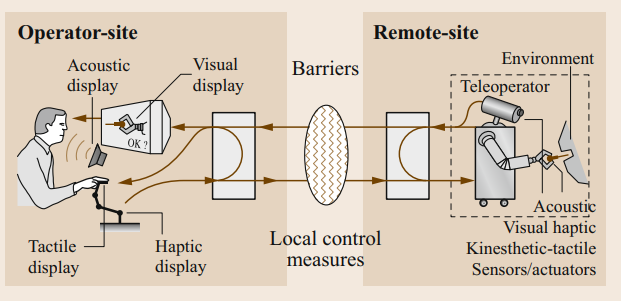
\includegraphics[scale=0.6]{Figures/Chapter2/teleoperation.png}
    \caption[telerobotic system]{telerobotic system}
    \label{fig:telerobotic system}
\end{figure}


\subsection{Telerobotic Architecture}
The architecture of a telerobotic system is a critical factor in determining the effectiveness, safety, and usability of the system. The architecture defines the interaction between the human operator and the teleoperator, the distribution of control tasks, and the level of autonomy in the system. The choice of architecture depends on the specific task requirements, the complexity of the environment, the operator's expertise, and the capabilities of the teleoperator.
There are three architectures structures for telerobotic systems, each with distinct characteristics and applications:
\begin{itemize}
    \item\textbf{Direct Control:} Direct Control is the simplest form of teleoperation, where every action taken by the human operator is directly translated into movements or actions of the teleoperator. This one-to-one correspondence means that the operator has immediate and complete control over the teleoperator's actions. Direct control systems are highly dependent on the operator's skill and attention, as there is minimal to no automation involved. This architecture is most effective in environments where precise, real-time control is necessary, and the task complexity is manageable by the human operator without additional automated support.

    \item\textbf{Shared Control:} Shared Control represents a more advanced teleoperation approach, where control is divided between the human operator and autonomous system functions. In this architecture, the operator and the teleoperation system share the task of controlling the teleoperator. The distribution of control can be dynamic, with the level of automation adjusting based on the task complexity, operator workload, or other contextual factors. Shared control systems are designed to combine human cognitive abilities with the precision and reliability of automated systems, optimizing task performance and potentially reducing operator fatigue. This approach is particularly beneficial in complex or unpredictable environments, where human judgment is essential, but so is the efficiency and consistency of automated processes.

    \item\textbf{Supervisory Control:} Supervisory Control takes a step further in integrating automation into teleoperation. In this architecture, the human operator takes on a supervisory role, monitoring the operation and intervening only when necessary. The teleoperator, equipped with a higher degree of autonomy, can perform tasks independently based on pre-programmed instructions or algorithms. The operator's primary responsibilities include setting goals, specifying constraints, monitoring progress, and intervening in case of unexpected events or system failures. Supervisory control is well-suited for operations in highly dangerous or inaccessible environments, or for tasks that require extended periods, where continuous direct human control is impractical.

\end{itemize}

%----------------------------------------------------------------------------------------
%	SECTION 2
%----------------------------------------------------------------------------------------

\section{Shared Control}
\label{Chapter2/PerspProj}
The adopted architectur to infer the teleoperation of the robotic arm is the shared control one, aiming to combine human cognitive capabilities with robotic efficiency to reduce the operator's workload and enhance task performance.\\
This architecture is pivotal in scenarios where fully autonomous robotic control is unfeasible due to unpredictable and complex environments.\\ 
More specifically, there are three main ways to implement the shared control architectur: Semi-Autonomous Control (SAC), State-Guidance Shared Control (SGSC), and State-Fusion Shared Control (SFSC).

\begin{itemize}
    \item\textbf{Semi-Autonomous Control (SAC):}In SAC the division of control tasks between the human operator and the autonomous system is distinctly demarcated. In this approach, the autonomous system and the human operator control separate variables, allowing each to leverage their strengths for improved task execution. This delineation enables the human operator to focus on high-level decision-making and strategic task elements, while the autonomous system manages the execution of routine or precise actions.\\ 
    The SAC model is particularly beneficial in complex and dynamic environments where human intuition and strategic oversight are crucial for success but are complemented by the precision and reliability of autonomous robotic actions. It facilitates a collaborative interaction where the operator's cognitive load is reduced, and the efficiency and safety of operations are enhanced by offloading specific control tasks to the robotic system

    \item\textbf{State-Guidance Shared Control (SGSC):} In SGSC the autonomous system provides direct guidance to the human operator, which can take various forms such as visual, auditory, or haptic feedback. This guidance is designed to assist the operator in making more informed decisions or in executing tasks with greater precision.\\ 
    The key principle behind SGSC is to enhance the operator's situational awareness and to facilitate the decision-making process without overtaking the human's control. This is achieved by allowing the autonomous system to suggest or warn the operator based on the system's perception and analysis of the environment or the task at hand. SGSC strategies are particularly useful in scenarios where human intuition and judgment are critical, but where the complexity or danger of the task necessitates additional inputs that can augment human capabilities. By providing guidance, SGSC aims to reduce the cognitive load on the operator, improve task performance, and enhance safety without diminishing the human's role in the control loop

    \item\textbf{State-Fusion Shared Control (SFSC):} SFSC  strategy goes beyond merely dividing tasks or providing guidance; it integrates the intentions and control signals of the human operator and the robot through a fusion mechanism. The fusion process often involves sophisticated algorithms that can weigh the contributions of the human and the robot based on factors like task complexity, operator expertise, and system capabilities. \\
    The goal of SFSC is to harness the strengths of both human and machine: the adaptability, judgment, and intuition of the human, alongside the precision, reliability, and speed of the machine. This integrated approach allows for a more seamless and efficient execution of tasks, particularly in environments that are too complex for fully autonomous robotics or require a level of decision-making beyond current autonomous capabilities. By dynamically adjusting the level of influence between human and machine based on real-time feedback and task requirements, SFSC strategies ensure that the control system remains adaptable and responsive to the nuances of each specific operation. This not only improves the performance and safety of telerobotic systems but also enhances the user experience by creating a more intuitive interaction between the human operators and the robotic system.

\end{itemize}
\begin{figure}[ht]
    \centering
    \begin{subfigure}[a]{0.32\textwidth}
      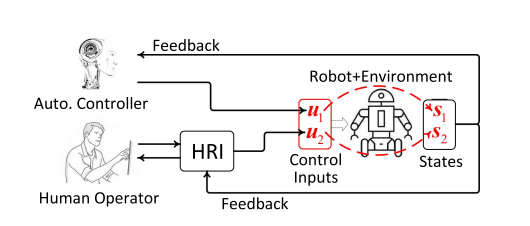
\includegraphics[width=\textwidth]{Figures/Chapter2/shared_1.png}
      \caption{Semi-Autonomous Control}
      \label{fig:semi_auto_control}
    \end{subfigure}
    \hfill % This will add horizontal space between the figures
    \begin{subfigure}[b]{0.32\textwidth}
      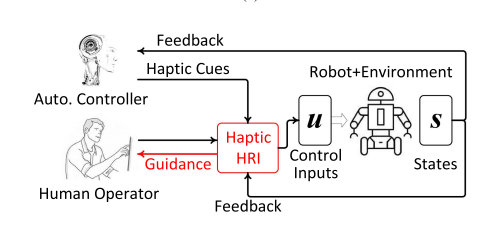
\includegraphics[width=\textwidth]{Figures/Chapter2/shared_2.png}
      \caption{Cooperative Control}
      \label{fig:cooperative_control}
    \end{subfigure}
    \hfill % This will add horizontal space between the figures
    \begin{subfigure}[c]{0.32\textwidth}
      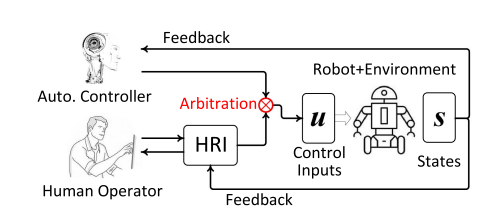
\includegraphics[width=\textwidth]{Figures/Chapter2/shared_3.png}
      \caption{Supervised Autonomous Control}
      \label{fig:supervised_auto_control}
    \end{subfigure}
    \caption{Types of Shared Control}
    \label{fig:shared_control_types}
  \end{figure}
  
In the context of this project the share controll architecture is implemented through the SFSC strategy. Since the aim is to help the teleoperator during teleoperation, this strategy ensures that the human operator and the robotic system can work together seamlessly, leaving the operator in control of the task while providing the necessary support and assistance to enhance task performance and safety.\\
To properly implement the strategy, the problem has to suibdivided into three main compartements: intention recognition, guidance and autonomous control.





%----------------------------------------------------------------------------------------
%	SECTION 3
%----------------------------------------------------------------------------------------\\     
\section{Intention Recognition}
The core challenge of intention recognition lies in accurately inferring the user's goals from a set of possible actions, often in real-time and under uncertainty. This process involves the collection and analysis of data generated by human actions, which could be in the form of physical movements, verbal commands, or control signals. The ultimate aim is to enable robots or autonomous systems to anticipate the needs or next actions of their human partners, allowing for proactive assistance.

\subsection{Metodologies}

Intention recognition methodologies span a range of approaches, reflecting the diversity of applications and the complexity of interpreting human intent.\\
At this day, there isn't a single, universally accepted method for intention recognition that applies across all scenarios in the teleoperation of robotic arms. Instead, the field comprises a variety of techniques, each with its strengths and limitations, tailored to specific contexts, tasks, and environments
\begin{itemize}
    \item\textbf{Probabilistic Models:} Techniques such as Hidden Markov Models (HMMs), as extensively explained in \cite{5480475} and \cite{AARNO2008692},is a statistical model that represents systems with probabilistic properties.
    It is characterized by its ability to model systems where the states are hidden and not directly observable, but the outcomes or observations associated with these states are observable.\\
    An HMM is defined by three primary elements: the state transition probability matrix $\textbf{A}$, which specifies the likelihood of transitioning from one state to another; the observation probability matrix $\textbf{B}$, detailing the probability of observing a certain symbol when in a specific state; and the initial state probability vector $\boldsymbol{\pi}$, indicating the likelihood of the system starting in each state.\\
    
    % Inserted TikZ Picture

    

    
    \begin{figure}[ht]
    \centering
    \begin{adjustbox}{center} 
    \begin{tikzpicture}
       
        % States
        \node[state] (s1) {$S_1$};
        \node[state] (s2) [right=of s1] {$S_2$};
        \node[state] (s3) [right=of s2] {$S_3$};
    
        % Observations
        \node[observation] (o1) [below=of s1] {$O_1$};
        \node[observation] (o2) [below=of s2] {$O_2$};
        \node[observation] (o3) [below=of s3] {$O_3$};
    
        % State transitions
        \draw[->] (s1) to[bend left] node[midway,above] {$a$} (s2);
        \draw[->] (s2) to[bend left] node[midway,above] {$a$} (s3);
        \draw[->] (s1) to[loop above] node[midway,above] {$a$} (s1);
        \draw[->] (s2) to[loop above] node[midway,above] {$a$} (s2);
        \draw[->] (s3) to[loop above] node[midway,above] {$a$} (s3);
    
        % Observations
        \draw[->] (s1) -- (o1) node[midway,left] {$b$};
        \draw[->] (s2) -- (o2) node[midway,left] {$b$};
        \draw[->] (s3) -- (o3) node[midway,right] {$b$};
    
        % Initial state probabilities
        \draw[->] ([xshift=-1cm]s1.west) -- (s1) node[midway,above] {$\pi$};
    \end{tikzpicture}
    \end{adjustbox}
    \hspace{5mm}
    \begin{adjustbox}{valign=t}
        % Legend
    \begin{minipage}[b]{0.4\textwidth}
            %\flushright % Adjusts the alignment of the legend to the right
            \textbf{Legend:}\\
            S: State\\
            O: Observation\\
            $a$: Transition Probability\\
            $b$: Observation Probability\\
            $\pi$: Initial State Probability
    \end{minipage}
    \end{adjustbox}
    \label{fig:Representation of a Hidden Markov Model (HMM)}
    \caption{Representation of a Hidden Markov Model (HMM)}
    \end{figure}
    
    As outlined in , while the application of HMMs in intention recognition for teleoperated robotic arm manipulation offers notable advantages in handling temporal dynamics and model flexibility, it concurrently presents substantial challenges, particularly in the necessity for precise and well-documented a priori knowledge.
    The complex nature of human decision-making processes complicates the task of accurately predicting operator behavior at each timestep of the teleoperation task; this is evident in the methodology, where the transition matrix $\textbf{A}$ is constructed based on empirical observations. This approach results in a relatively simplistic policy for state transitions, potentially oversimplifying the nuanced and variable nature of human intent during teleoperation tasks.
    





    \item\textbf{Inverse Reinforcement Learning (IRL):} Inverse Reinforcement Learning (IRL) is a sophisticated method for deciphering and forecasting the intentions behind human operators' actions in teleoperation, where understanding complex decision-making is key to enhancing human-robot interactions.\\
    Brian D. Ziebart et al.~\cite{ziebart2008maximum} extend IRL's capabilities through a probabilistic framework grounded in the maximum entropy principle, adept at navigating the uncertainties in teleoperation decision-making. 
    This approach, by favoring the least biased action distribution based on observed behaviors, provides a refined representation of operators' reward functions, thus accurately modeling their intent.\\
    The incorporation of maximum entropy IRL into intent recognition significantly improves how robotic systems can preemptively adjust to and fulfill human operator goals, shifting from merely reactive to proactive adaptations.
    Despite these advancements, implementing IRL in real-time applications is hindered by the extensive computational resources needed to process complex data and infer human intent in a fast and accurate manner, presenting a challenge in the practical deployment of IRL-enhanced robotic systems.
    
    \item\textbf{Partially Observable Markov Decision Processes (POMDPs):} Partially Observable Markov Decision Processes (POMDPs) are a class of decision-making models that consider situations where the state of the system is partially observable or uncertain to the decision-maker. 
    In a POMDP framework, the decision-maker must rely on observations that may provide indirect or incomplete information about the system's state to make decisions. 
    This model extends the Markov Decision Process (MDP) framework by incorporating a layer of uncertainty regarding the system's actual state, making it particularly suited for complex environments where full information is not available.\\
    In the context of shared control systems, POMDPs play a crucial role in modeling the interaction between a human user and an autonomous system, especially when the system's understanding of the user's intent is uncertain.
    the authors in \cite{doi:10.1177/0278364918776060} delve into this by formalizing shared autonomy as a POMDP, which assists in minimizing the expected cost-to-go with an unknown goal.
    This approach acknowledges that while the autonomous system may not confidently predict the user's specific goal until it is nearly achieved, it can still offer valuable assistance by optimizing actions that are generally helpful across multiple potential goals.
    When the system has high confidence in a single user goal, the framework focuses assistance more narrowly to support that specific objective. This balance allows for more effective and adaptive assistance, even in the face of uncertainty about the user's exact intentions.\\
    Despite its great ability to handle uncertainty, give focused help based on goals, and use hindsight optimization to make real-time processing better, this method still encounters problems with how complex its computations are, requiring substantial computational resources to function effectively.
    Additionally, the performance of this approach is deeply interconnected with the precision of its observational models for accurately perceiving and interpreting actions. 
    Inaccurate models significantly impair the system's capability to discern the user's intentions, leading to challenges in providing timely and relevant assistance. 
    Therefore, it is crucial to enhance the accuracy of these models to ensure they accurately reflect real-world scenarios, thereby optimizing the method's efficiency

    \item\textbf{Recurrent neural networks:} Recurrent Neural Networks (RNNs) are a specialized type of artificial neural networks crafted to recognize and interpret patterns in sequential data, including but not limited to text, genomic sequences, handwriting, or numerical time series from various sensors. What sets RNNs apart from traditional feedforward neural networks is their unique architecture featuring directed cycles in their connections.
    This design allows them to retain information over time, enabling the network to maintain a form of 'memory'.
    Such a capability is invaluable for tasks where understanding the context or the sequence in which data points appear is crucial.
    By iterating through elements in a sequence and maintaining a state that accumulates information seen thus far, RNNs effectively process sequences by leveraging their internal state (memory) to manage a range of inputs sequentially. This characteristic renders them incredibly useful for a variety of applications, including language modeling, speech recognition, and forecasting in time series data.
    Despite their advantages, RNNs are not without their challenges. Notably, they can be difficult to train effectively due to issues like vanishing and exploding gradients, which hinder their ability to learn long-range dependencies within the data.\\
    As elaborated in \cite{10.1162/neco_a_01199} to overcome these obstacles, Long Short-Term Memory (LSTM) networks emerge as a powerful solution within the domain of shared control of robotic arms, especially for tasks like intention prediction. 
    The LSTM, with its unique ability to learn and remember over long periods, has significantly improved the predictability and accuracy of user intention in shared control systems. This advanced form of RNN addresses the core limitations of its predecessors by efficiently handling long-term dependencies. 
    The robustness of Long Short-Term Memory (LSTM) networks against time gaps in data input, coupled with their capacity to adapt to individual user preferences, significantly boosts the efficiency and personalization of shared control systems.
    However, the sophisticated nature of LSTMs brings about challenges, including increased computational complexity and a greater need for extensive training data. Despite these challenges, the integration of LSTMs into Recurrent Neural Network (RNN) technology marks a significant leap forward. 
    It expands the potential for more intuitive and adaptable human-robot collaboration within shared control environments, navigating through the practical difficulties associated with their implementation.
\end{itemize}



%----------------------------------------------------------------------------------------
%	SECTION 4
%----------------------------------------------------------------------------------------
\section{Guidance}
In the domaine of shared control systems, guidance embodies a sophisticated integration of feedback and control strategies, facilitating seamless and intuitive interactions between humans and robots.
At the heart of guidance lies the objective to harmonize the decision-making capabilities and adaptability of human operators with the accuracy, reliability, and operational efficiency of robotic systems. 
This harmony is achieved through a continuous exchange of information, where the system furnishes the human operator with immediate, pertinent data, feedback, and actionable advice. 
This enables the operator to make well-informed decisions that guide the robot's actions. Such a reciprocal flow of information significantly enhances the effectiveness of task performance, elevates safety standards, and guarantees an advanced level of control and adaptability.
This acts as a critical link between human operators and automated systems, effectively reducing the workload.%-----------------------------------
%	SUBSECTION 1
%-----------------------------------
\subsection{Metodologies}

Guidance methodologies in shared control systems showcase a broad spectrum of approaches, highlighting the complex interplay between human operators and robotic mechanisms, especially in teleoperation scenarios;among these, Artificial Potential Fields (APF), the Dynamic Window Approach (DWA), the Vector Field Histogram (VFH), and Rapidly-exploring Random Trees (RRT) have been proven to be particularly effective in guiding robotic systems in shared control environments.\\

\begin{itemize}
    \item\textbf{Artificial Potential Fields (APF):} 
    The implementation of Artificial Potential Fields (APF) \cite{100007} is integral to enhancing real-time shared control in teleoperation frameworks, focusing on obstacle avoidance and efficient path planning. 
    APF employs virtual forces that guide the robotic system by creating a potential field where obstacles generate repulsive forces, and the goal exerts an attractive force. This dynamic allows the robot to navigate by following the gradient of the potential function, akin to traversing a landscape of peaks and valleys designed to steer clear of obstacles while being drawn toward the target.
    Upon setting a goal, APF aligns the robot's movement with the operator's intent by modulating these virtual forces, thereby facilitating an intuitive interaction between the human operator and the robotic system.\\
    The primary challenges associated with APF include the robot's susceptibility to getting trapped in local minima—regions where the potential gradient is zero, preventing further movement towards the goal—and the method's purely reactive nature to collision avoidance. 
    In standard APF applications, the robot alters its course only when in close proximity to obstacles, which may not be efficient for advanced navigation and obstacle avoidance in cluttered environments. 

    However, as presented in \cite{9734752}, the problem of obstacle avoidance in cluttered environments can be efficiently overcome with the dynamic generation of escape points around obstacles. 
    These escape points are designed to help the robotic system bypass obstacles smoothly while avoiding the pitfalls of local minima.\\ 
    This approach not only addresses the issue of the robot getting stuck but also allows for more proactive obstacle avoidance by modifying the robot's trajectory in advance, rather than merely reacting when close to obstacles.

    \item\textbf{Dynamic Window Approach (DWA):} he Dynamic Window Approach (DWA) is a fundamental technique in mobile robotics, utilized for motion planning and obstacle avoidance in dynamic environments. 
    It operates by constraining the robot's velocity to a "dynamic window," considering its current state and capabilities. 
    Within this window, potential velocities are evaluated using a cost function that incorporates factors such as obstacle distance, goal direction, and robot velocity. 
    By selecting the velocity that maximizes this function while ensuring collision-free navigation, the DWA facilitates rapid decision-making in real-time motion control.\\ 
    To fit this method to a shared control contex, in \cite{7932524} a novelty method has been developed. 
    Building upon DWA principles, the Biomimetical Dynamic Window Approach (BDWA) integrates human navigation behaviors into robotic motion planning. 
    This extension aims to generate robot movement resembling human path preferences, enhancing user interaction with assistive devices.\\ 
    BDWA achieves this by selecting velocities aligning with human-like paths, guided by a reward function assessing trajectory resemblance. 
    Through iterative refinement, BDWA balances safe navigation with human-like movement, optimizing the shared control experience in assistive technologies.\\ 


\end{itemize}    

